% Gemini theme
% https://github.com/anishathalye/gemini
%
% We try to keep this Overleaf template in sync with the canonical source on
% GitHub, but it's recommended that you obtain the template directly from
% GitHub to ensure that you are using the latest version.

\documentclass[final]{beamer}

% ====================
% Packages
% ====================

\usepackage[T1]{fontenc}
\usepackage{lmodern}
\usepackage[size=a1,scale=1.15]{beamerposter}
\usetheme{gemini}
\usecolortheme{gemini}
\usepackage{graphicx}
\usepackage{booktabs}
\usepackage{tikz}
\usepackage{pgfplots}
\usepackage{graphicx}
\usepackage{booktabs}
\usepackage[position=top]{subfig}
\usepackage{lipsum}

\usepackage[skins,xparse]{tcolorbox}
% ====================
% Lengths
% ====================

% If you have N columns, choose \sepwidth and \colwidth such that
% (N+1)*\sepwidth + N*\colwidth = \paperwidth
\newlength{\sepwidth}
\newlength{\colwidth}
\setlength{\sepwidth}{0.025\paperwidth}
\setlength{\colwidth}{0.3\paperwidth}

\newcommand{\separatorcolumn}{\begin{column}{\sepwidth}\end{column}}

% ====================
% Title
% ====================

\title{%
  \texorpdfstring{%
    \makebox[\linewidth]{%
    \setlength{\parindent}{0pt}
      \makebox[0pt][l]{%
        \raisebox{\dimexpr-\height+\baselineskip-20pt}[0pt][0pt]
          {
\includegraphics[height=2.4\baselineskip]{nirma.jpg}}% Left logo
      }\hfill
      \makebox{Extreme Weather Prediction using Deep Learning}%
      \hfill\makebox[0pt][r]{%
        \raisebox{\dimexpr-\height+\baselineskip-20pt}[0pt][0pt]
          {
\includegraphics[height=2.4\baselineskip]{ISRO.png}}% Right logo
      }%
      \setlength{\parindent}{0pt}
    }%
  }
  {Extreme Weather Prediction using Deep Learning}} % Poster title
% \title{}

\author{Yash Thesia (15BCE126) \inst{1} \and Vidhey Oza (15BCE130) \inst{1} \and Dr. Priyank Thakkar \inst{1} \and Dr. Nitant Dube \inst{2}}

\institute[shortinst]{\inst{1} Institute of Technology, Nirma University \samelineand \inst{2} Space Application Centre, ISRO}


% ====================
% Body
% ====================

\begin{document}

\begin{frame}[t]
\begin{columns}[t]
\separatorcolumn

\begin{column}{.7\colwidth}

  \begin{alertblock}{Introduction}

   \begin{itemize} 

\item \textbf{Problem Statement}: An important scientific goal for climate researchers is weather nowcasting, which can be used effectively to predict extreme weather events. This problem of weather nowcasting can be formulated as the prediction of the next data point or frame in sequence, given a fixed window of sequence that precedes the said data point. Using these short-term predictions, the system should be able to identify areas where the cloud systems or humidity levels can lead to extreme conditions in the future. 

\item \textbf{Objective}: We propose a 2 phase deep learning pipeline. In the first phase, we nowcast frames captured by the INSAT-3D satellite sensors. In the second phase, we use these predictions to identify hotspots of meteorological variables that signal towards genesis of extreme weather events. 


\end{itemize}

  \end{alertblock}

  \begin{block}{Data}

     The complete data that we have worked on was captured using the INSAT-3D Imager sensor. In the first phase, we used the 6 channel standard disk products as given in Table 1.
     
    \begin{table}
\centering
\caption{L1B Standard Products (INSAT-3D). Used in Phase 1. }
\label{table:data:phase1}
\resizebox{\columnwidth}{!}{
\begin{tabular}{@{}clll@{}}
\toprule
\multicolumn{1}{c}{\begin{tabular}[c]{@{}c@{}}Sr.\\ No.\end{tabular}} & \multicolumn{1}{c}{\begin{tabular}[c]{@{}c@{}} Channel \\ Name\end{tabular}} & \multicolumn{1}{c}{\begin{tabular}[c]{@{}c@{}}Spatial\\Resolution\\\end{tabular}} & \multicolumn{1}{c}{Description} \\ \midrule
1 & IMG\_VIS & 1km & Rad. for Visible Channel \\
2 & IMG\_SWIR & 1km & Rad. for Shortwave Infrared Channel \\
3 & IMG\_TIR1 & 4km & B.T. for Thermal Infrared Channel 1 \\
4 & IMG\_TIR2 & 4km & B.T. for Thermal Infrared Channel 2 \\
5 & IMG\_MIR & 4km & B.T. for Middlewave Channel \\
6 & IMG\_WV & 8km & B.T. for Water Vapor Channel \\ \bottomrule
\end{tabular}
}
\end{table}

    This data consists of the L1B standard products that are used to derive geophysical products like hydro-estimator precipitation or land surface temperature is given in Table 2. The spatial resolution of the image in coordinates is 60$^{\circ}$N to 60$^{\circ}$S and 30$^{\circ}$E to 130$^{\circ}$E, with varying pixel based resolution as given in Table 1. The temporal resolution of the data is 30 minutes. 

    \begin{table}
\centering
\caption{Derived Products. Used in Phase 2. }
\label{table:data:phase2}
\resizebox{\columnwidth}{!}{
\begin{tabular}{cllll}
\toprule
\begin{tabular}[c]{c}Sr.\\ No.\end{tabular} & \multicolumn{1}{c}{Product Name} & \multicolumn{1}{c}{Resolution} & \multicolumn{1}{c}{Application} & \multicolumn{1}{c}{Dataset Period} \\ \midrule
1 & \begin{tabular}[c]{l}Hydro-Estimator\\ Precipitation\end{tabular} & 4km & \begin{tabular}[c]{l}Used for extreme \\ rainfall events\end{tabular} & \begin{tabular}[c]{l}July to \\ August 2018\end{tabular} \\ \midrule
2 & \begin{tabular}[c]{l}Land Surface\\ Temperature\end{tabular} & 4km & \begin{tabular}[c]{l}Used for extreme \\ heat events\end{tabular} & \begin{tabular}[c]{l}April to \\ May 2018\end{tabular} \\ \bottomrule
% 2 & \begin{tabular}[c]{@{}l@{}}Land Surface \\ Temperature\end{tabular} & 4km & \multirow{2}{*}{\begin{tabular}[c]{@{}l@{}}Used for heatwave events \\ and spatial correlation\end{tabular}} & \multirow{2}{*}{April to May} \\ \bottomrule
\end{tabular}
}
\end{table}

  \end{block}

\end{column}

\separatorcolumn

\begin{column}{1.3\colwidth}

  \begin{block}{Implementation Pipeline}
  
  \begin{center}
    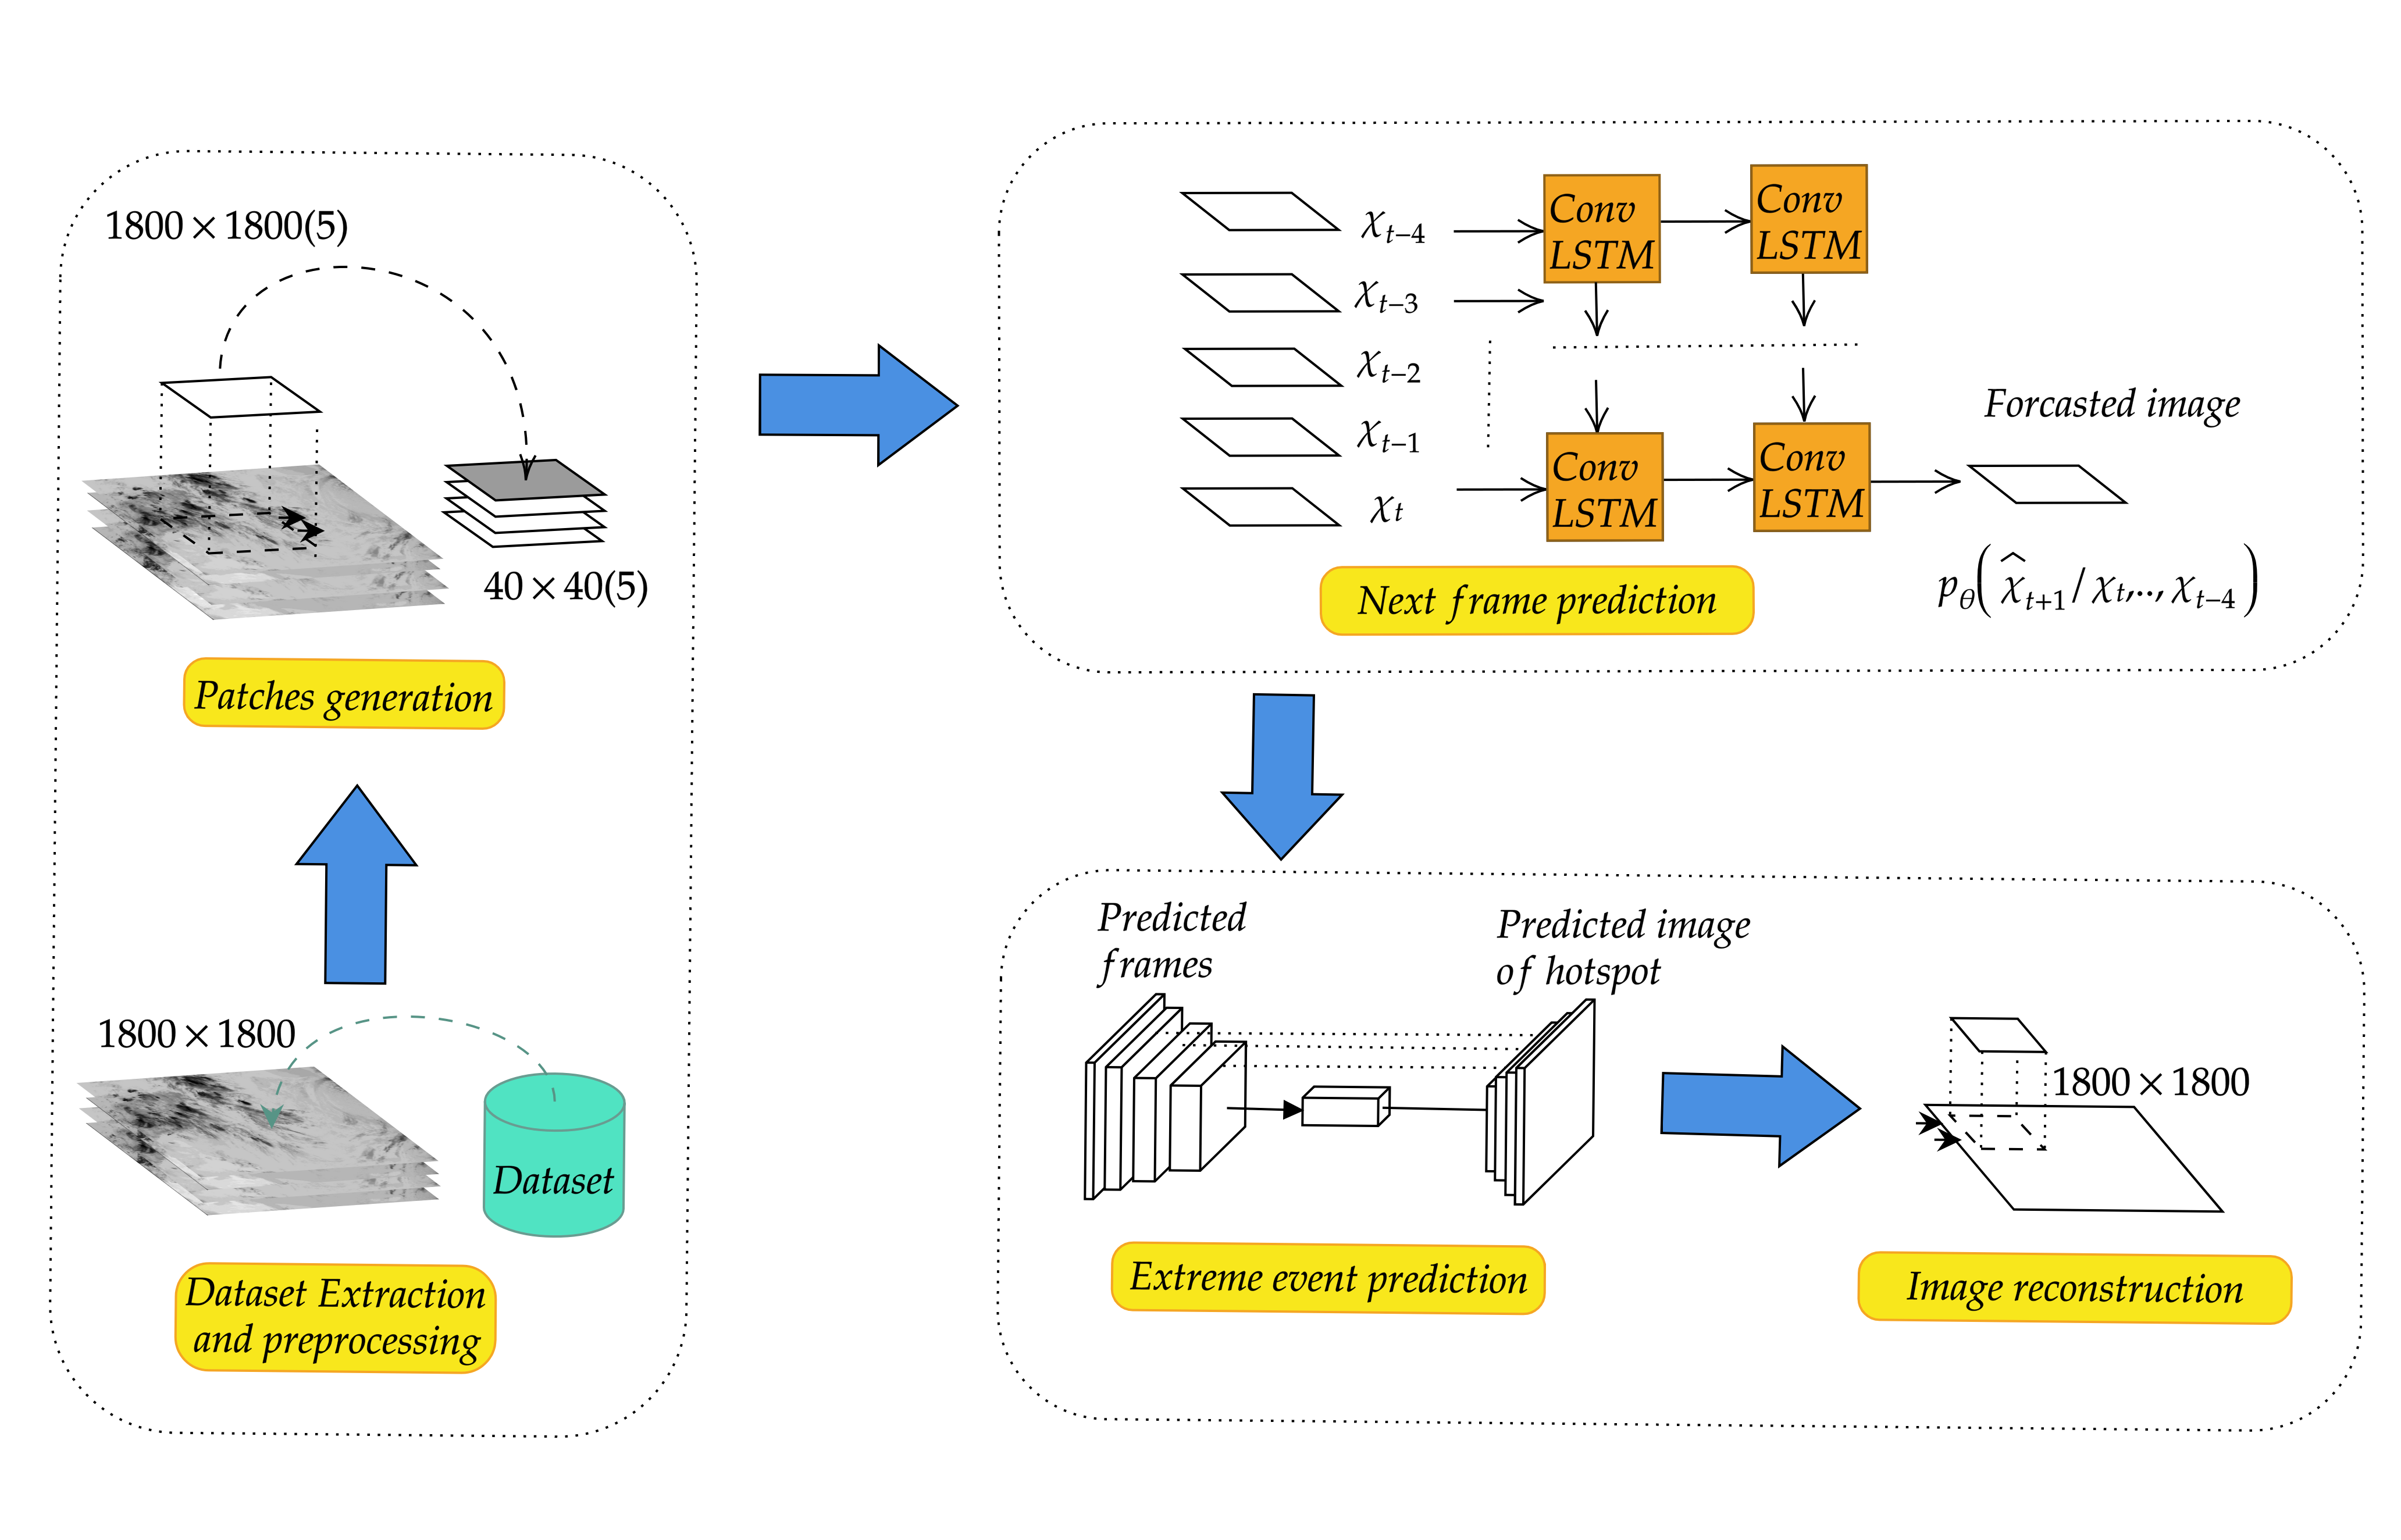
\includegraphics[width=0.7\columnwidth]{full.png}
    \end{center}
  
  
  \end{block}

  \begin{block}{Results}

    \begin{center}
    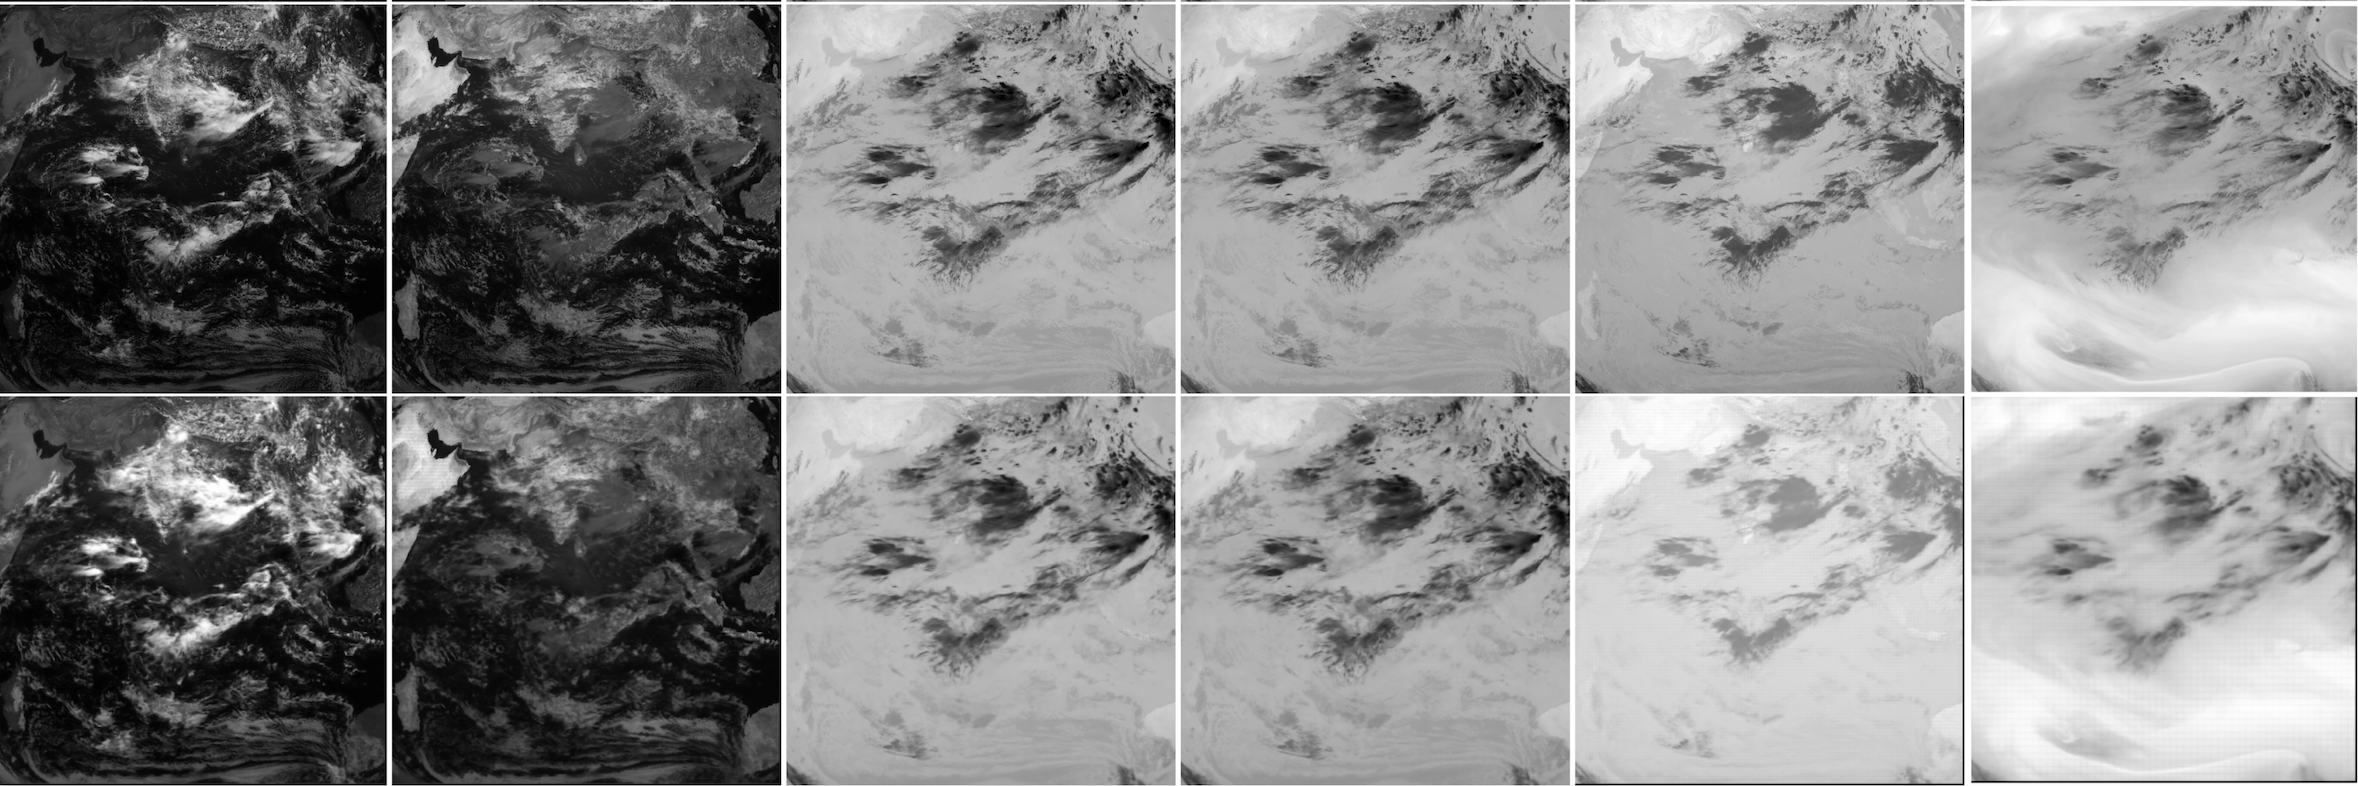
\includegraphics[width=0.7\columnwidth]{example-predictions-halfhour.jpg}
    
    Top to bottom:actual $(t+1)^{th}$ frame, predicted frame. Left to right: as listed in Table 1. 
    \end{center}  
    
    \begin{center}
    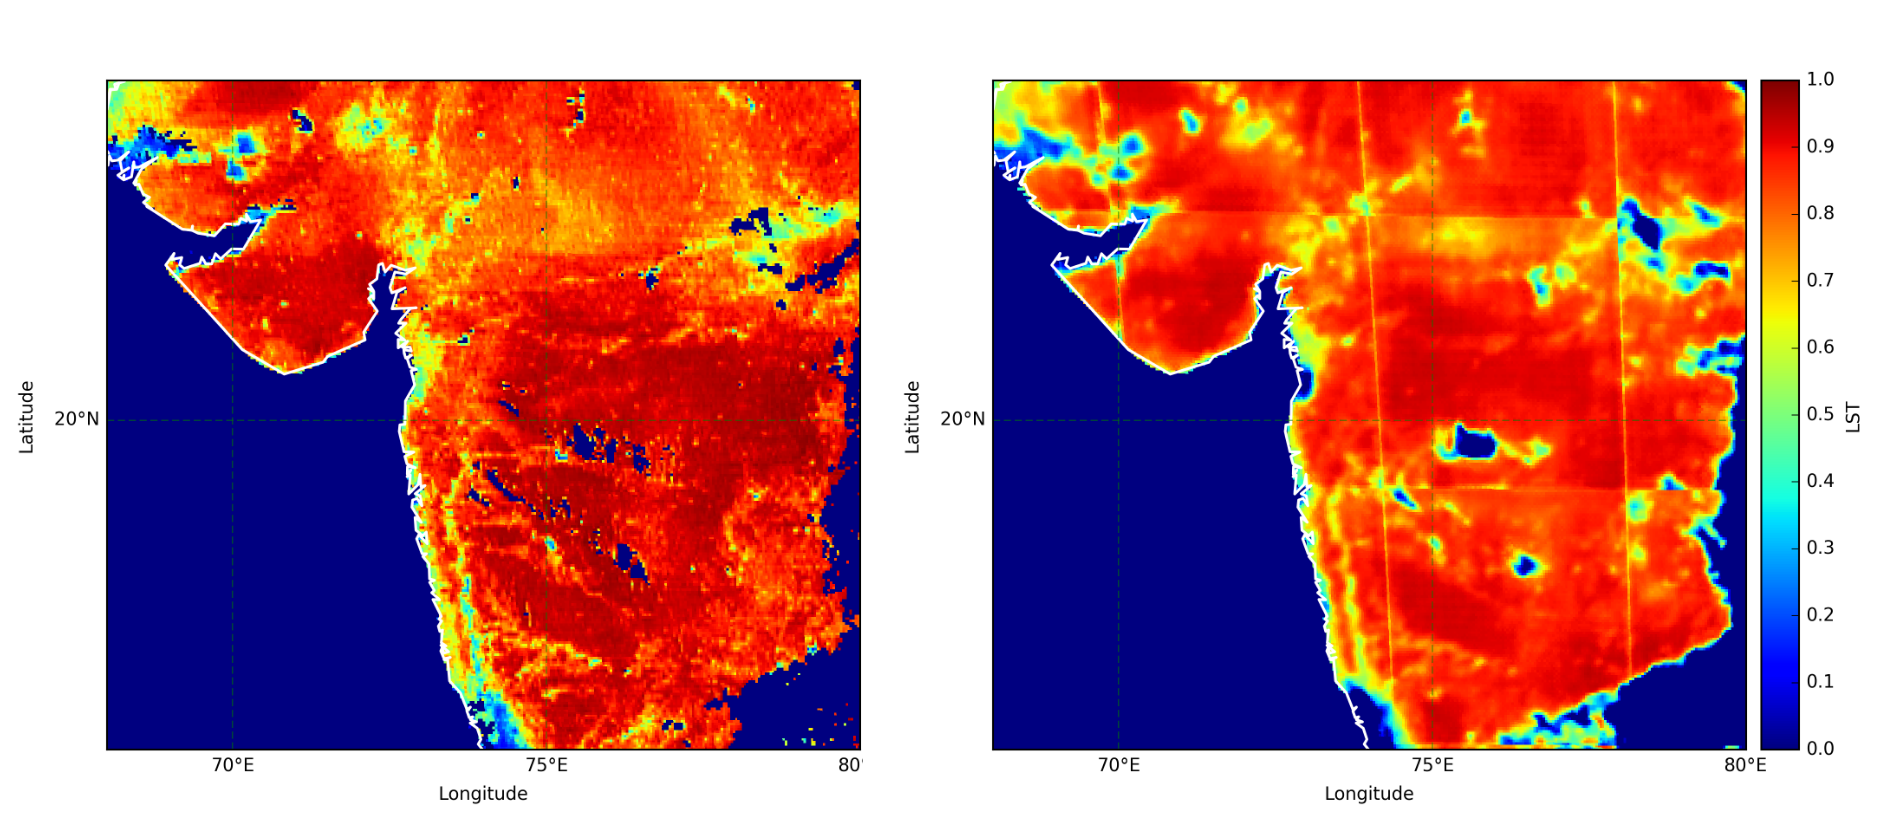
\includegraphics[width=0.53\columnwidth]{example-tem.png}
    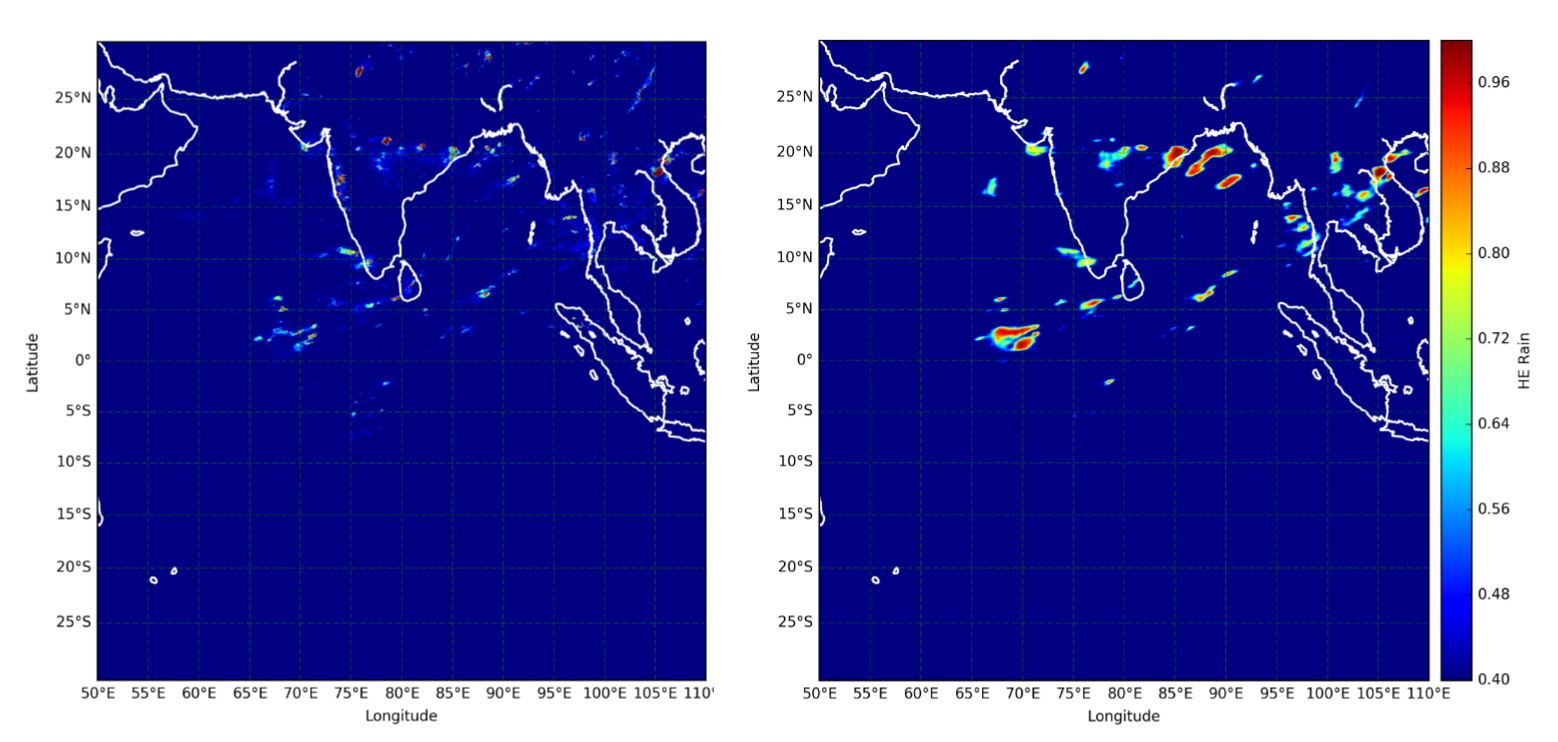
\includegraphics[width=0.47\columnwidth]{example-hem.png}
    
    Left: Actual, predicted $(t+1)^{th}$ LST frames. Right: Actual, predicted $(t+1)^{th}$ HE values. 
    \end{center}  
    
     \begin{center}
    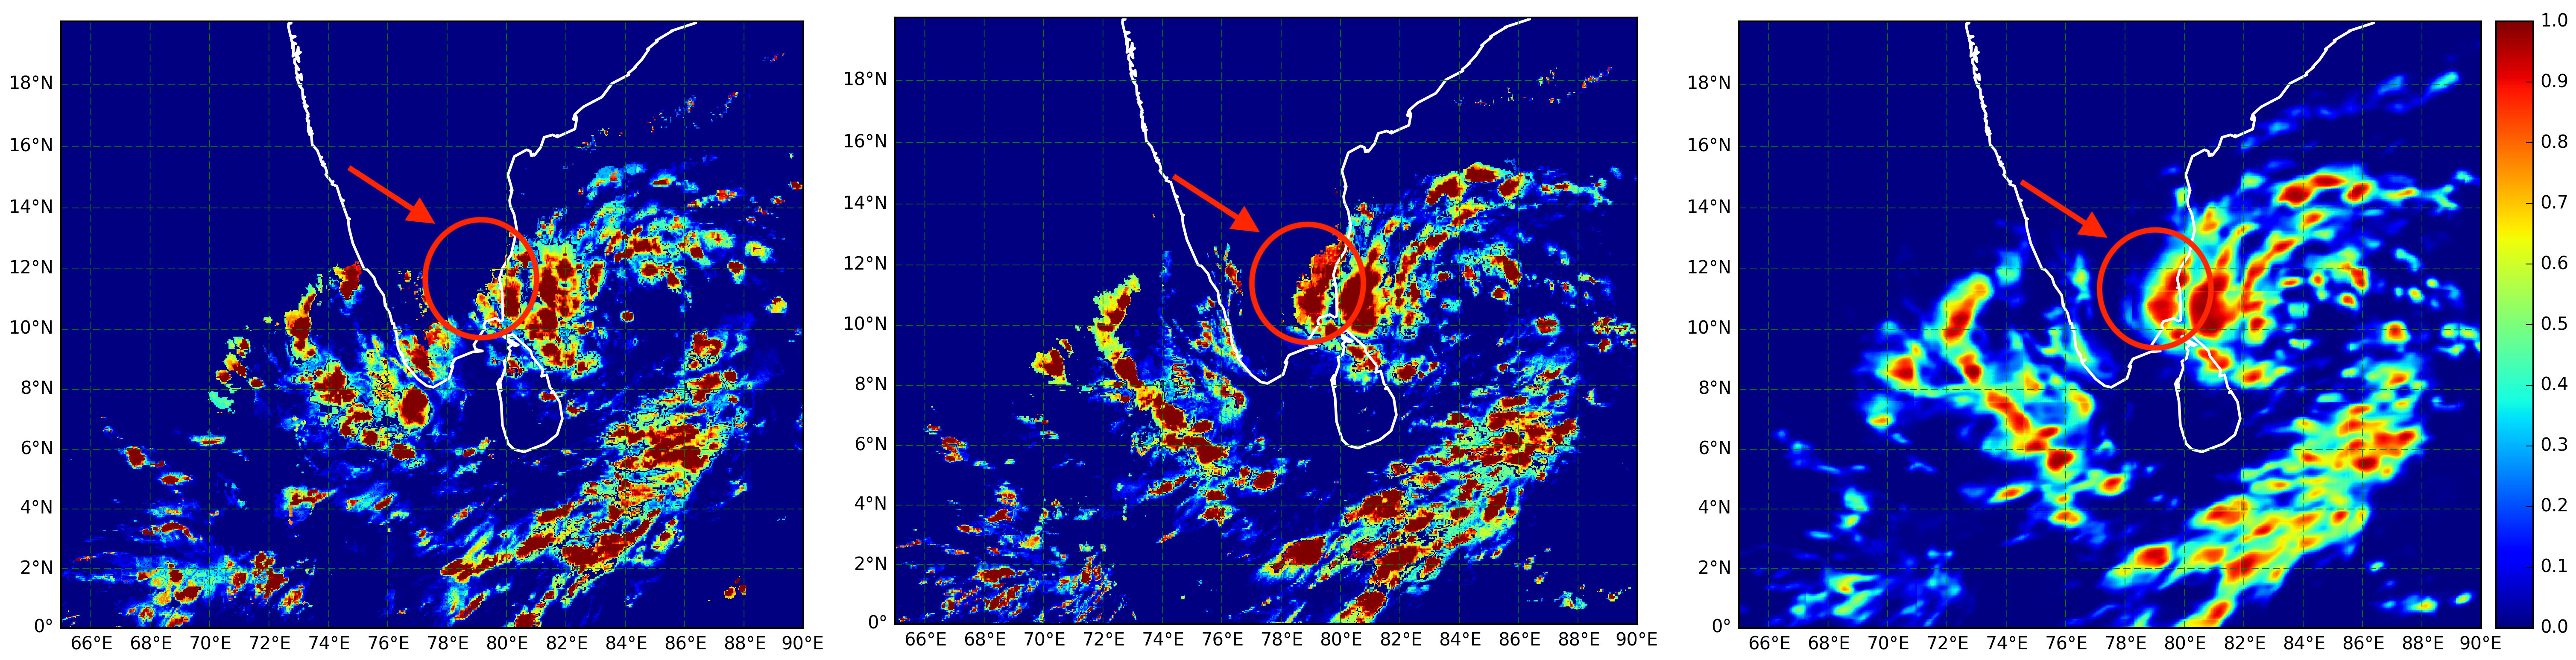
\includegraphics[width=0.7\columnwidth]{example-chennai.jpg}
    
    Left to right: $(t-4)^{th}$ frame, actual$(t+1)^{th}$ frame and predicted frame of HE rain on 8 November 2015 at Chennai
    \end{center}  
    
    
    % \caption{Left to right: $(t-4)^{th}$ input image, actual image and predicted image of hydro-estimator rain. }
  
\end{block}

\end{column}

\separatorcolumn

\begin{column}{0.9\colwidth}

\begin{block}{Dataset Preprocessing and Model}
For practical training purposes, we convert the full frames into patches of $40\times40$ with a stride of $20$. During reconstruction, we compute the pixel by overlapping and averaging the patches based on positioning. 

\textbf{Phase 1}: Given 5 sequence frames as input, predict next frames (+00:30, +01:00, +01:30, +02:00, +02:30) of all 6 channels sequentially. Model: ConvLSTM. Normalization: min-max scaling. Loss: binary cross-entropy. Optimizer: Adam. 

\textbf{Phase 2}: Given predicted images from Phase 1, predict the meteorological variable frame corresponding to given extreme event. Model: U-Net. Normalization: tanh (for extreme event classification). Loss: binary cross-entropy. Optimizer: Adam. 

\end{block}

\begin{block}{Results}

\begin{table}
\caption{Result metrics}
\centering
    \subfloat[Phase 1 results. ]{
        \label{table:results:phase1}
        % \begin{tabular}{@{}lll@{}}
        % \toprule
        % Dataset Channel  & SSIM  & PSNR   \\ \midrule
        % IMG\_VIS         & 0.852 & 25.413 \\
        % IMG\_SWIR        & 0.801 & 27.169 \\
        % IMG\_TIR1        & 0.916 & 22.034 \\
        % IMG\_TIR2        & 0.884 & 23.564 \\
        % IMG\_MIR         & 0.891 & 23.879 \\
        % IMG\_WV          & 0.963 & 26.327 \\ \bottomrule
        % \end{tabular}
        \begin{tabular}{clllll}
        \toprule
        Channels & \multicolumn{1}{c}{+00:30} & \multicolumn{1}{c}{+01:00} & \multicolumn{1}{c}{+01:30} & \multicolumn{1}{c}{+02:00} & \multicolumn{1}{c}{+02:30} \\ \midrule
        VIS & 28.264 & 26.053 & 24.598 & 23.929 & 24.066 \\
        SWIR & 27.538 & 24.921 & 22.358 & 20.404 & 20.200 \\
        TIR1 & 28.504 & 24.202 & 21.146 & 19.046 & 17.604 \\
        TIR2 & 31.239 & 28.481 & 26.447 & 24.747 & 23.256 \\
        MIR & 26.178 & 22.210 & 19.275 & 17.084 & 15.443 \\
        WV & 31.100 & 27.970 & 25.384 & 23.822 & 22.565 \\ \midrule
        Avg. & 28.804 & 25.639 & 23.201 & 21.505 & 20.522 \\ \bottomrule
        \end{tabular}
    }
    \quad
    \subfloat[Phase 2 results. ]{
        \label{table:results:phase2}
        \begin{tabular}{@{}lll@{}}
        \toprule
        \begin{tabular}[c]{@{}l@{}}Extreme event\\ parameters\end{tabular} & SSIM  & PSNR  \\ \midrule
        Hydro-Estimator & 0.923 & 24.36 \\ 
        Land Surface Temperature & 0.803 & 22.96 \\ \bottomrule
        \end{tabular}
    }
\end{table}

\end{block}
  
\begin{block}{Scope \& Future Work}
Apart from the direct benefit of being able to forecast the next-hour weather, we explore the advantages of being able to extract derived features like hydro-estimator rain or surface temperature. Hence, we explore the possibility of a prediction system that can predict any feature of the next half-hour and next hour, given the underlying standard feature set. 

As future work, we can focus on the slow processing of the ConvLSTM as the three dimensional processing with gated properties. So, we can replace the ConvLSTM with U-Net for faster results by slightly reducing accuracy. 

\end{block}

\begin{block}{Acknowledgements}
We would like to thank Dr. Nitant Dube who has been exceptionally positive and helpful in the journey of SMART program at SAC-ISRO. We are grateful to Dr. Priyank Thakkar and Dr. Sanjay Garg for always giving the right direction and encouraging us to innovate. We are thankful to SAC-ISRO for providing delightful opportunity and facilitating environment. 


\end{block}

\end{column}

\separatorcolumn
\end{columns}
\end{frame}

\end{document}
